\documentclass[aspectratio=169,11pt]{beamer}
\usetheme{Madrid}
\usecolortheme{default}

\usepackage{amsmath,amssymb}
\usepackage{booktabs}
\usepackage{graphicx}
\usepackage{hyperref}

\title{Presentation I: Basics}
\subtitle{Physics-Aware Action-Conditioned World Modeling for Billiards}
\author{Your Name}
\date{\today}

\begin{document}

\begin{frame}
  \titlepage
\end{frame}

\begin{frame}{Why This Project?}
\begin{itemize}
  \item Goal: generate interactive billiards rollouts conditioned on user actions.
  \item Key challenge: not just visual quality, but physical logic over time.
  \item Physics checks:
  \begin{itemize}
    \item do balls bounce correctly off walls?
    \item do collisions look physically plausible?
    \item do object identities stay consistent over rollout?
  \end{itemize}
\end{itemize}
\end{frame}

\begin{frame}{Pipeline Overview}
\begin{enumerate}
  \item Data generation from simulator:
  \begin{itemize}
    \item frames \(x_t\), actions \(a_t\), simulator state \(s_t\)
  \end{itemize}
  \item VAE compresses frames to latents \(z_t\)
  \item Action-conditioned DiT predicts next-latent diffusion noise
  \item Rollout eval at horizons \(h=\{1,4,8,16,32\}\)
  \item Interactive inference route for click/drag actions
\end{enumerate}
\end{frame}

\begin{frame}{Data Scale (v1 + v2 + v3)}
\begin{itemize}
  \item v1: \(100{,}000\) episodes (baseline coverage)
  \item v2: \(100{,}000\) episodes (higher diversity)
  \item v3: \(200{,}000\) episodes (collision-heavy)
  \item 600 frames per episode \(\Rightarrow\) 400k episodes total
\end{itemize}
\vspace{0.3em}
\centering
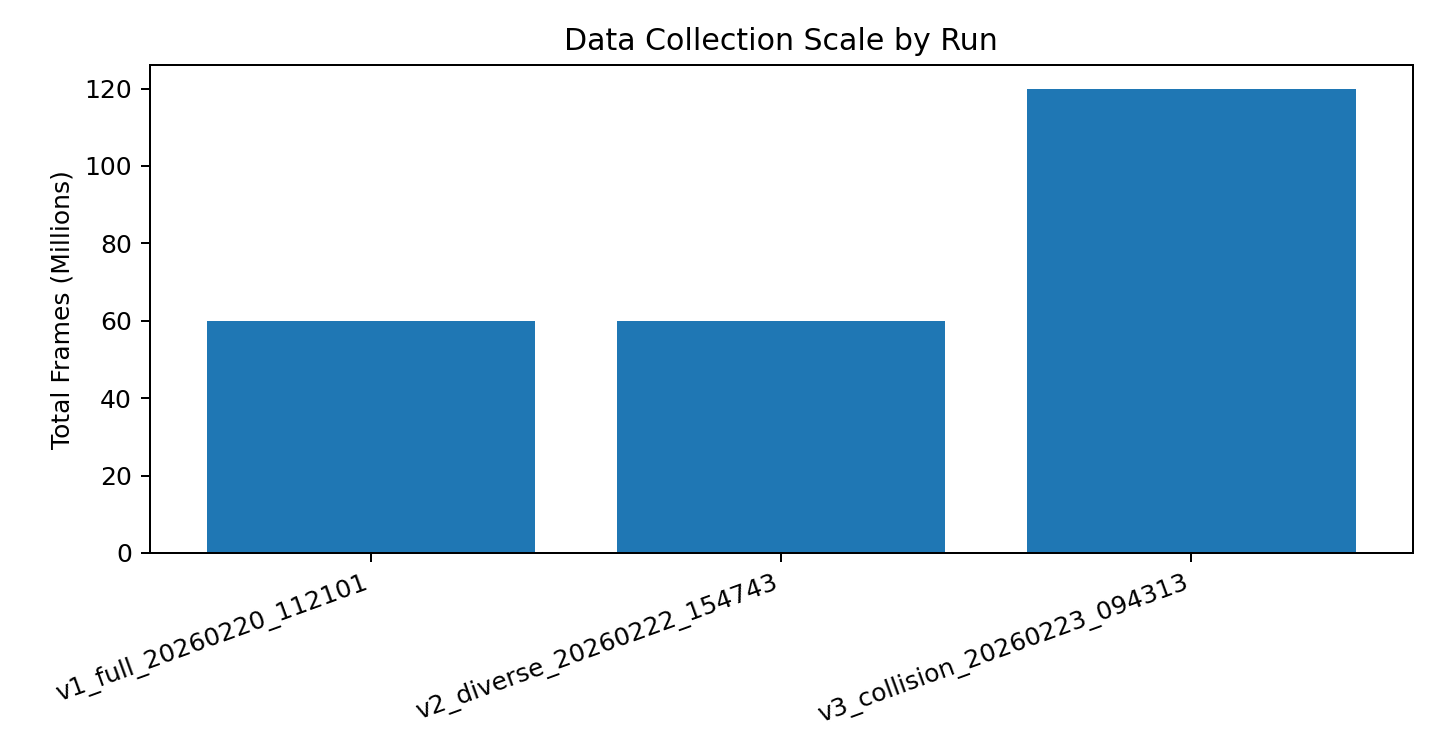
\includegraphics[width=0.72\linewidth]{../../milestones_preview/charts/data_collection_scale_frames_millions.png}
\end{frame}

\begin{frame}{VAE Stage (Compression)}
\begin{itemize}
  \item Input frame: \(72 \times 128 \times 3\)
  \item Latent: \(4 \times 9 \times 16\) (\(\sim 48\times\) element compression)
  \item Why: makes large-scale world-model training feasible.
\end{itemize}
\vspace{0.4em}
\[
\mathcal{L}_{\text{VAE}} =
\lambda_{L1}\|x-\hat{x}\|_1
 + \lambda_{\text{LPIPS}}\mathcal{L}_{\text{LPIPS}}
 + \lambda_{\text{KL}}\mathcal{L}_{\text{KL}}
\]
\centering
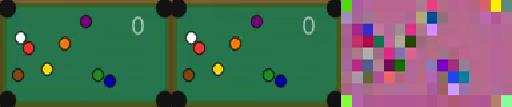
\includegraphics[width=0.75\linewidth]{../final_project_essay/assets/vae_latent_compare_ep0_13s.png}
\end{frame}

\begin{frame}{Diffusion Model Basics}
Forward corruption in latent space:
\[
x_\tau = \sqrt{\bar\alpha_\tau}x_0 + \sqrt{1-\bar\alpha_\tau}\epsilon,\quad \epsilon\sim\mathcal{N}(0,I)
\]
Model predicts noise \(\hat\epsilon_\theta\):
\[
\mathcal{L}_{\text{base}} = \mathbb{E}\|\hat\epsilon_\theta - \epsilon\|_2^2
\]
\vspace{0.3em}
Reconstruct predicted clean latent:
\[
\hat x_0 = \frac{x_\tau - \sqrt{1-\bar\alpha_\tau}\hat\epsilon_\theta}{\sqrt{\bar\alpha_\tau}}
\]
\end{frame}

\begin{frame}{Action-Conditioned DiT}
\begin{itemize}
  \item Context window: \(z_{t-L+1:t}\), with \(L=8\)
  \item Action vector: \(a_t = [f_x,f_y,\text{trigger}]\)
  \item Model predicts next-latent diffusion noise conditioned on context + action
\end{itemize}
\vspace{0.4em}
\[
\hat\epsilon_t = f_\theta(z_{t-L+1:t}, a_t, x_\tau, \tau)
\]
\begin{itemize}
  \item Inference uses DDIM sampling for speed/quality tradeoff.
\end{itemize}
\end{frame}

\begin{frame}{Diffusion Forcing (Core Idea)}
\begin{itemize}
  \item Baseline trains mostly one-step.
  \item Rollout inference is multi-step autoregressive.
  \item Diffusion forcing trains multi-step with scheduled teacher forcing.
\end{itemize}
\[
\mathcal{L}_{\text{DF}} = \frac{1}{K}\sum_{k=1}^K \|\hat\epsilon_k-\epsilon_k\|_2^2
\]
\[
\tilde z_{k+1}=m_k z_{k+1}^{gt} + (1-m_k)\hat x_{0,k},\quad m_k\sim \text{Bernoulli}(p_{tf}(n))
\]
\begin{itemize}
  \item This reduces train/inference mismatch and helps long-horizon stability.
\end{itemize}
\end{frame}

\begin{frame}{Evaluation Protocol}
\begin{itemize}
  \item Fixed-horizon rollout metrics at \(h=\{1,4,8,16,32\}\)
  \item Latent metrics: MSE, MAE
  \item Frame metrics (after VAE decode): PSNR, L1
  \item Important: metric ``@16'' means exactly step-16 prediction, not average over 1..16
\end{itemize}
\end{frame}

\begin{frame}{Takeaway for Deck II}
\begin{itemize}
  \item Deck I covered: data, VAE, diffusion, DiT, DF, and evaluation setup.
  \item Deck II will answer:
  \begin{itemize}
    \item Did diffusion forcing actually improve interactive physics?
    \item Where does the model still fail?
    \item What are the concrete next steps?
  \end{itemize}
\end{itemize}
\end{frame}

\end{document}
